\chapter{Evaluation}
\label{ch:evaluation}

\section{Success criteria}

\paragraph{Success Criterion}
The original project proposal (\Aref{ch:proposal}) stated the following three criteria for success:
\begin{enumerate}
    \item 
        Implement SGC and extract the concepts used for each of the synthetic datasets.
        \label{crit1}
    \item 
        Implement GCN and extract the concepts to use as a baseline.
        \label{crit2}
    \item 
        Compare the concepts between SGC and GCN using the metrics of concept completeness and concept purity.
        \label{crit3}
\end{enumerate}

\emph{I meet all three success criteria.}
In addition to the above project success criteria, and to aid the analysis of SGC compared to GCN, the two models are compared using mean \emph{test accuracy}.

\paragraph{Meeting criterion 1}
\Sref{sec:datasets-imp} detais the implementation of the SGC pre-computation and \Sref{sec:reproduction} verifies the correctness of the implementation.
\Sref{sec:comp-concept} demonstrates concept extraction on the synthetic datasets.

\paragraph{Meeting criterion 2}
\Sref{sec:models} details the implementation of the GCN model.
\Sref{sec:reproduction} verifies the correctness of the GCN implementation and demonstrates concept extraction.

\paragraph{Meeting criterion 3}
\Sref{sec:concepts} details the implementation of concept extraction, calculation and visualisation.
\Sref{sec:comp-concept} demonstrate the comparison of SGC and GCN using the metrics of concept completeness and purity.
Additionally, \Sref{sec:comp-acc} demonstrates further comparison between the models using the metric of model accuracy.

\section{Methodology}

\subsection{Hyperparameters}
\label{sec:hyperparameters}

\paragraph{Reproduction}
\textit{Magister et al.}\cite{magister2021gcexplainer} use a GCN model to evaluate their proposed graph concept explainer.
The paper trains and evaluates the model on the same 5 synthetic node classification datasets described in \Sref{sec:synth} and therefore the same hyperparameters are used for the GCN baseline.

\textit{Wu et al.}\cite{wu2019simplifying} states that the weight decay parameter for the Planetoid\cite{kipf2016semi} datasets was found using \texttt{hyperopt}\cite{bergstra2013making} over 60 iterations.
This process was repeated for results reproduction however it was found that the hyperparameters for the learning rate were different from those stated.

The hyperparameters for these models are available in tables \ref{tab:GCN-params} and \ref{tab:SGC-reproduction-params}.
Additionally the concept extraction metrics are presented in table \ref{tab:GCN-concept-params}.

%\begin{table}
    \centering
    \begin{tabular}{c|ccc}
        \textbf{Dataset} &
        \textbf{Layers} &
        \textbf{Learning rate} &
        \textbf{Epochs} \\
        \midrule
        BA Shapes       & 3 $\times$ 20 & 0.001 & 3000 \\
        BA Grid         & 3 $\times$ 20 & 0.001 & 3000 \\
        BA Community    & 6 $\times$ 50 & 0.001 & 6000 \\
        Tree Cycles     & 3 $\times$ 50 & 0.001 & 7000 \\
        Tree Grid       & 7 $\times$ 20 & 0.001 & 10000 \\
        \midrule \\
        REDDIT BINARY   & 4 $\times$ 40 & 0.005 & 3000 \\
        Mutagenicity    & 4 $\times$ 30 & 0.005 & 10000 \\
    \end{tabular}
    \caption{GCN hyperparameters from table 15 in \textit{Magister et al.}\cite{magister2021gcexplainer}. All models use \texttt{ReLU}\note{citation needed?} activation functions between layers with a single linear layer classifier with \texttt{softmax}\note{citation needed?}.}
    \label{tab:GCN-params}
\end{table}


%\begin{table}[h]
    \centering
    \captionsetup{width=.9\textwidth}
    \begin{tabular}{c|cccc}
        \textbf{Dataset} &
        \textbf{Degree} &
        \textbf{Learning rate} &
        \textbf{Weight decay} &
        \textbf{Epochs} \\
        \midrule
        Cora        & 2 & 0.002 & 0.04 & 100 \\
        Citeseer    & 2 & 0.004 & 0.08 & 100 \\
        PubMed      & 2 & 0.0005 & 0.25 & 100 \\
    \end{tabular}
    \caption{SGC hyperparameters using \texttt{hyperopt}\cite{bergstra2013making} as proposed by \textit{Wu et al.}\cite{wu2019simplifying}. All models use \texttt{softmax}.}
    \label{tab:SGC-reproduction-params}
\end{table}


%\begin{table}[h]
    \centering
    \captionsetup{width=.9\textwidth}
    \begin{tabular}{c|cc}
        \textbf{Dataset} &
        \textbf{Clusters (k)} &
        \textbf{Receptive field (n)} \\
        \midrule
        BA Shapes       & 10 & 2 \\
        BA Grid         & 10 & 3 \\
        BA Community    & 30 & 2 \\
        Tree Cycles     & 10 & 3 \\
        Tree Grid       & 10 & 3 \\
        \midrule
        REDDIT BINARY   & 20 & 1 \\
        Mutagenicity    & 30 & 3 \\
    \end{tabular}
    \caption{Concept extraction parameters used in \textit{Magister et al.}\cite{magister2021gcexplainer}.}
    \label{tab:GCN-concept-params}
\end{table}



\paragraph{New models}
The core project defines 5 models based on the SGC architecture as required by criterion \ref{crit1}.
As the underlying graph operator is the same for both GCN and SGC the degree of the SGC model same as the layers in the equivalent GCN model.
This is the approach that \textit{Wu et al.}\cite{wu2019simplifying} take to creating there SGC models.

The learning rate for SGC models is likely to be different from the GCN models due to the reformulation.
Furthermore, \textit{Wu et al.}\cite{wu2019simplifying} use weight decay to keep weight values close to $0$ as would be assumed from the multiplication of weight matrices in equation \ref{eq:theta}.
Rather than stochastic approaches to finding hyperparameters a sweep of values is tested.

The result of these searches is presented in figures \ref{fig:SGC-surfaces} and \ref{fig:JSGC-surfaces}.
The majority of sweeps demonstrate minimal impact on model accuracy and therefore a learning rate of $0.01$ and weight decary constant of $0.1$ is chosen.
The hyperparameters used are presented in table \ref{tab:SGC-params}.

%\begin{table}
    \centering
    \begin{tabular}{c|cccc}
        \textbf{Dataset} &
        \textbf{Degree} &
        \textbf{Learning rate} &
        \textbf{Weight decay} &
        \textbf{Epochs} \\
        \midrule
        BA Shapes       & 3 & 0.01 & 0.1 & 3000 \\
        BA Grid         & 3 & 0.01 & 0.1 & 3000 \\
        BA Community    & 6 & 0.001 & 0.1 & 6000 \\
        Tree Cycles     & 3 & 0.01 & 1.0 & 7000 \\
        Tree Grid       & 7 & 0.01 & 0.01 & 10000 \\
    \end{tabular}
    \caption{SGC hyperparameters based on the corresponding GCN hyperparameters in \ref{tab:GCN-params} and using the results of the hyperparameter search in \note{reference when added}. All models use \texttt{softmax}\note{citation needed?}.}
    \label{tab:SGC-params}
\end{table}



\paragraph{Datasets}
The batch sizes for all the datasets match those described in \textit{Ying et al.}\cite{ying2019gnnexplainer} and \textit{Kipf et al.}\cite{kipf2016semi}.
The number of epochs for each dataset matches those proposed in \textit{Magister et al.}\cite{magister2021gcexplainer} and \textit{Wu et al.}\cite{wu2019simplifying} or until convergence for SGC.

\subsection{Model Evaluation}
\label{sec:evaluation}

\paragraph{Concept evaluation}
Criterion \ref{crit3} requires evaluation of the models with respect to concept purity and completeness.
These metrics are discussed in \Sref{sec:GCE} and implementation is described in \Sref{sec:concepts}.
As well as quantitative analysis concepts lend themselves to qualitative analysis which focuses on visual similarities between the two models.
The qualitative analysis will also help in understanding the differences in how the two architectures work.

For qualitative analysis only BA Shapes and Mutagenicity will be covered in detail; brief analysis of the other datasets is presented in \Aref{app:concepts}.
This extends to extensions where only a subset of datasets are trained on as a proof of concept.

It is important to note a number of drawbacks of the GCExplainer in comparing two different models quantitatively.
\begin{enumerate}
    \item 
        Concept purity is calculated only using subgraphs with less than 13 nodes.
        This means that pure quantitative analysis does not represent a full comparison of the two models.
    \item 
        The number of clusters and the receptive field of the concepts can be arbitrarily manipulated to find the highest score.
        To combat this the new SGC models are compared against the same concept extraction parameters presented in table \ref{tab:GCN-concept-params}.
    \item 
        \label{nb:accuracy}
        \textit{Ying et al.}\cite{ying2019gnnexplainer} only suggest concept extraction for models that achieve an accuracy of atleast $95\%$ on synthetic datasets. 
\end{enumerate}

%The full comparison of concepts requires a qualitative analysis of the extracted concepts.
%The concepts produced by SGC can be analysed in isolation to infer how SGC reasons about graphs.
%These can then be compared to the concepts produced by GCN to highlight the differences in reasoning and which is easier to understand.
%When reproducing results this is done by comparing the analysis suggested by \textit{Magister et al.}\cite{magister2021gcexplainer} to the reproduced concepts.
%Furthermore, a visual comparison of the concepts can be made, such as matching published concepts to reproduced concepts.

\paragraph{Accuracy evaluation}
Drawback \ref{nb:accuracy} motivates the additional evaluation metric of accuracy as \Sref{sec:comp-acc} demonstrates that SGC does not meet the desired accuracy.
To achieve this each synthetic dataset is split into a train and test set using an 80:20 split.
Note that TUDataset\cite{Morris+2020} and Planetoid\cite{kipf2016semi} use there own train/test splits.

The synthetic datasets are generated randomly along with the train/test split and thus each random seed produces a new variation of the synthetic dataset.
This means that using the same seeds across different experiments results in the same train/test split.
This also means that although the hyperparameter search evaluates parameters on the test split of a dataset as different as used the evaluation test nodes are unseen.

\subsection{Confidence intervals}
\label{sec:reporting}
The mean accuracy across 10 different initiliasations is reported using $\mu = \sum_i\frac{\text{accuracy}_i}{10}$ as an unbiased estimator of the mean.
The confidence interval of each of the runs uses the unbiased standard deviation estimator $\sigma = \sqrt{\sum_i(\text{accuracy}_i - \mu)/(10 - 1)}$.
For experiments where very high variance is present outliers are removed based on the median, $m$, and the interquartile range, $\text{ITR}$, of the accuracies.\footnote{In the cases where outliers are removed the estimators are adjusted accordingly.}
An outlier is defining as being outside the range $[m - 1.5 \times \text{ITR}, m + 1.5 \times \text{ITR}]$.


\subsection{Reproducibility}
\error{Return to at the end to make sure that all aspects are met.}

\subsection{System specifications}
The experiments are not resource-intensive due to the incredibly small datasets and so carrying out the hyperparameter search and multiple final runs can be completed on my personal machine.
My machine has an AMD Ryzen 7 5700U CPUs @ 1.8GHz with 16 cores wuth 15 Gigabytes of RAM.
The machine does have an AMD ATI Lucienne GPU but due to the fact that \texttt{PyTorch Geometric}\cite{paszke2019pytorch} did not support RoCM I was unable to utilise this.

To speed up the retrieval of experimental results for extensions I utilised a Google Colab Pro account with 1 hyperthreaded Intel Xeon Processor @ 2.3GHz with 1 core and 12 Gigabytes of Ram.
The account also has access to a Tesla K80 GPU with 12GB of RAM.

\note{Include figures demonstrating system use later.}

\section{Results Reproduction}
\label{sec:reproduction}

As discussed in \Sref{sec:testing} the testing strategy includes the reproduction of prior results from \textit{Magister et al.}\cite{magister2021gcexplainer} on GCN and \textit{Wu et al.}\cite{wu2019simplifying} on SGC.
I reproduce all of the experiments from \textit{Magister et al.} and the Planetoid\cite{kipf2016semi} from \textit{Wu et al.} as these are most relevant.

\paragraph{Success criterion}
\Sref{sec:GCN-reproduction} demonstrates an implementation of GCN trained on the synthetic datasets with concept extraction.
Tables \ref{tab:GCN-acc} and \ref{tab:GCN-concepts} and figure \ref{fig:GCN-BA-Shapes} demonstrate the results achieved.
This fulfills the \ref{crit2}$^{nd}$ success criterion.

\paragraph{Method}
In both cases across all datasets the hyperparameters presented in tables \ref{tab:GCN-params} and \ref{tab:SGC-reproduction-params} are used.
Each model, dataset experiment is run 10 times with different randomly pre-selected seeds and the mean and confidence interval are presented in accordance with \Sref{sec:reporting}.
The implementation of SGC pre-computation is presented in \Sref{sec:datasets-imp}.
The implementation of GCN uses the layers provided by \texttt{PyTorch Geometric}\cite{Fey/Lenssen/2019}.

\subsection{SGC}
\begin{table}
    \centering
    \begin{tabular}{c|cc}
        \multicolumn{1}{c}{\textbf{Dataset}} &
        \multicolumn{1}{c}{\textbf{Wu et al.}} &
        \multicolumn{1}{c}{\textbf{My results}} \\
        \midrule
        Cora        & 81.0\% $\pm$ 0.0 & 80.0\% $\pm$ 0.1 \\
        Citeseer    & 71.9\% $\pm$ 0.1 & 71.4\% $\pm$ 0.1 \\
        Pubmed      & 78.9\% $\pm$ 0.0 & 71.3\% $\pm$ 2.1 \\
    \end{tabular}
    \caption{Reproduction of experiments from table 2 in \textit{Wu et al.}\cite{wu2019simplifying}. The mean accuracy of 10 experiment runs is taken using hyperparameters found by \texttt{hyperopt}\note{citation needed}.}
    \label{tab:SGC-reproduction}
\end{table}



Table \ref{tab:SGC-reproduction} presents the accuracy achieved by my SGC models compared to the accuracy presented in table 2 of \textit{Wu et al.}\cite{wu2019simplifying}.
As can be seen in both Cora and Citeseer the accuracies are closely correlated, though the accuracy presented by \textit{Wu et al.} are outside of my confidence interval.
Comparitively Pubmed presents a large discrepancy between the published results and the reproduced results with large variation in the reproduced results.
These descrepancies are likely due to the uncertainty in hyperparameters as the exact weight decay constant used is unknown.
Furthermore, the published learning rate of 0.2 yields worse results and so, as demonstrated in table \ref{tab:SGC-reproduction-params}, new learning rates are used.
Based on these considerations I consider my implementation of SGC to be correct.

\subsection{GCN}
\label{sec:GCN-reproduction}
\paragraph{Accuracy}
\begin{table}
    \centering
    \begin{tabular}{c|cc}
        \multicolumn{1}{c}{\textbf{Dataset}} &
        \multicolumn{1}{c}{\textbf{Magister et al.}} &
        \multicolumn{1}{c}{\textbf{My results}} \\
        \midrule
        BA Shapes       & 95.6\% & 98.0\% $\pm$ 2.2 \\
        BA Grid         & 99.0\% & 99.5\% $\pm$ 0.7 \\
        BA Community    & 95.7\% & 86.3\%\tablefootnote{\label{nb:epochs1}Using the same epochs stated in \textit{Magister et al.}\cite{magister2021gcexplainer}. More epochs yields a closer value.} $\pm$ 3.3 \\
        Tree Cycles     & 96.0\% & 95.8\% $\pm$ 3.2 \\
        Tree Grid       & 95.1\% & 92.5\% $\pm$ 5.4 \\
        \midrule
        REDDIT BINARY   & 89.1\% & 89.1\% $\pm$ 2.2 \\
        Mutagenicity    & 93.0\% & 93.8\% $\pm$ 1.6 \\
    \end{tabular}
    \caption{Reproduction of experiments from table 16 in \textit{Magister et al.}\cite{magister2021gcexplainer}. The mean test accuracy of 10 experiment runs is taken using \textit{Magister et al.}'s hyperparameters.}
    \label{tab:GCN-acc}
\end{table}


Table \ref{tab:GCN-acc} presents the accuracy achieved the reproduced GCN models compared to the accuracy published in table 16 of \textit{Magister et al.}\cite{magister2021gcexplainer}.
As can be seen in the majority of cases the reproduced accuracy matches or exceeds the accuracy presented by \textit{Magister et al.}.
Given the small size of the synthetic datasets it is expected that near 100\% accuracy is achieved.
For the real-world datasets the expectation is above 85\% as suggested by \textit{Ying et al.}\cite{ying2019gnnexplainer}.

BA Community is a significant outlier in the results reaching neither near 100\% or the suggested 95\%.
However, if the model is allowed to train for more than the defined 6000 epochs an accuracy closer to 95\% is achieved.
Due to these considerations I consider my implementation of GCN to be correct.

\paragraph{Concept scores}
\begin{table}
    \centering
    \begin{tabular}{c|cccc}
        \multirow{2}{*}{\textbf{Dataset}} &
        \multicolumn{2}{c}{\textbf{Magister et al.}} &
        \multicolumn{2}{c}{\textbf{My results}} \\
        &
        \textbf{Completeness} & 
        \textbf{Purity} & 
        \textbf{Completeness} & 
        \textbf{Purity} \\
        \midrule
        BA Shapes       & 0.964 & 3.375 & 0.929 & 0.000 \\
        BA Grid         & 1.000 & 4.923 & 1.000 & 0.000 \\
        BA Community    & 0.678 & 0.000 & 0.623 & 5.600 \\
        Tree Cycles     & 0.949 & 1.167 & 0.970 & 4.391\\
        Tree Grid       & 0.965 & 3.100 & 0.951 & 1.417\\
        \midrule
        REDDIT BINARY   & 0.713 & 6.968 & 0.746 & 1.429 \\
        Mutagenicity    & 0.967 & 5.400 & 0.626 & 0.375 \\
    \end{tabular}
    \caption{Reproduction of experiments from tables 4 and 5 in \textit{Magister et al.}\cite{magister2021gcexplainer}. The activation space for each experiment selected from the best performing model is used with the mean purity score presented.}
    \label{tab:GCN-concepts}
\end{table}


Table \ref{tab:GCN-concepts} presents the concept scores for each of the top performing GCN models compared to those in tables 4 and 5 in \textit{Magister et al.}.
As with the accuracy reproduction the values for concept completeness are closely correlated for the majority of the models.
%\fig{erroneous-labels}{A subset of the concepts discovered for Mutagenicity highlighting the erroneous labels. Each row represents a concept and the graphs are coloured according to standard chemical colouring.}
%
%Figure \ref{fig:erroneous-labels} demonstrates that the clustering for Mutagenicity focuses on chemical similarity which does not necessarily correlate to mutagen similarity.
%This means that the concept completeness is likely to be low as demonstrated in \ref{tab:GCN-concepts} though the actual model accuracy may be high.
However, average purity has little correlation between the two results which is due to the 13 node cut-off and non-deterministic nature of $k$-Means clustering.
%rather than an incorrect implementation.


\begin{figure}
    \centering
    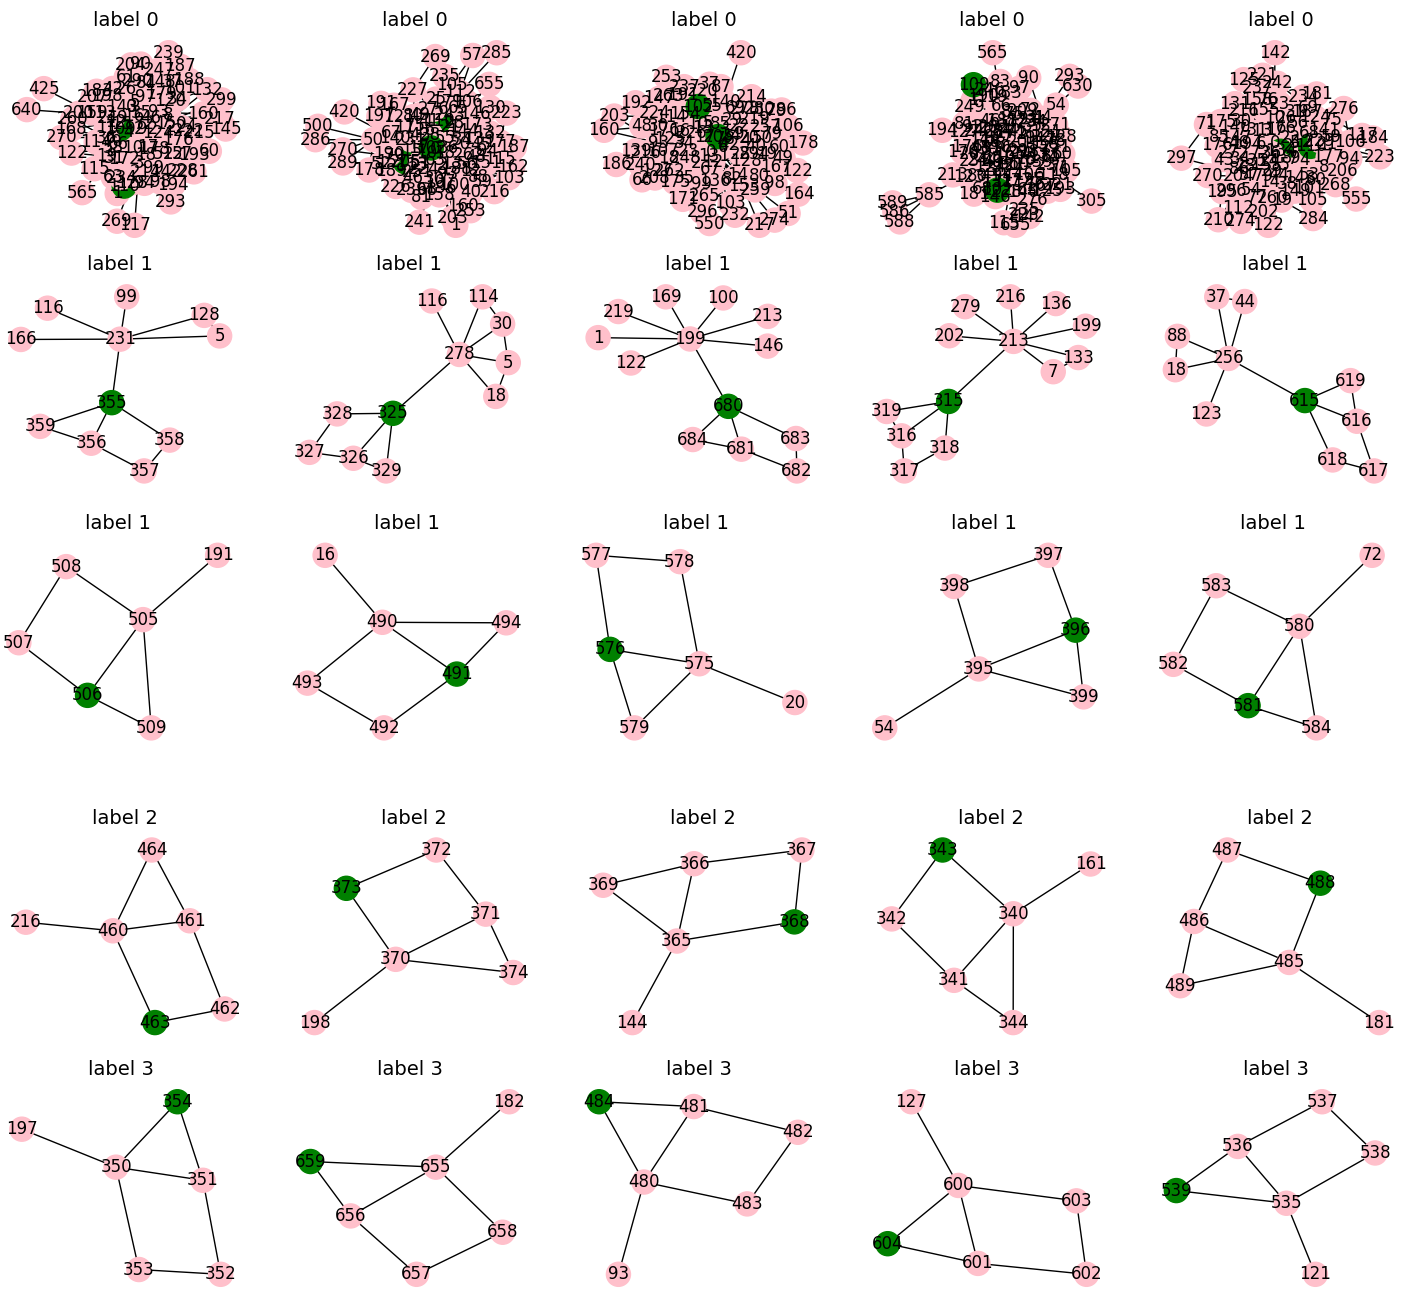
\includegraphics[width=0.45\textwidth]{figures/GCN-BA-Shapes}
    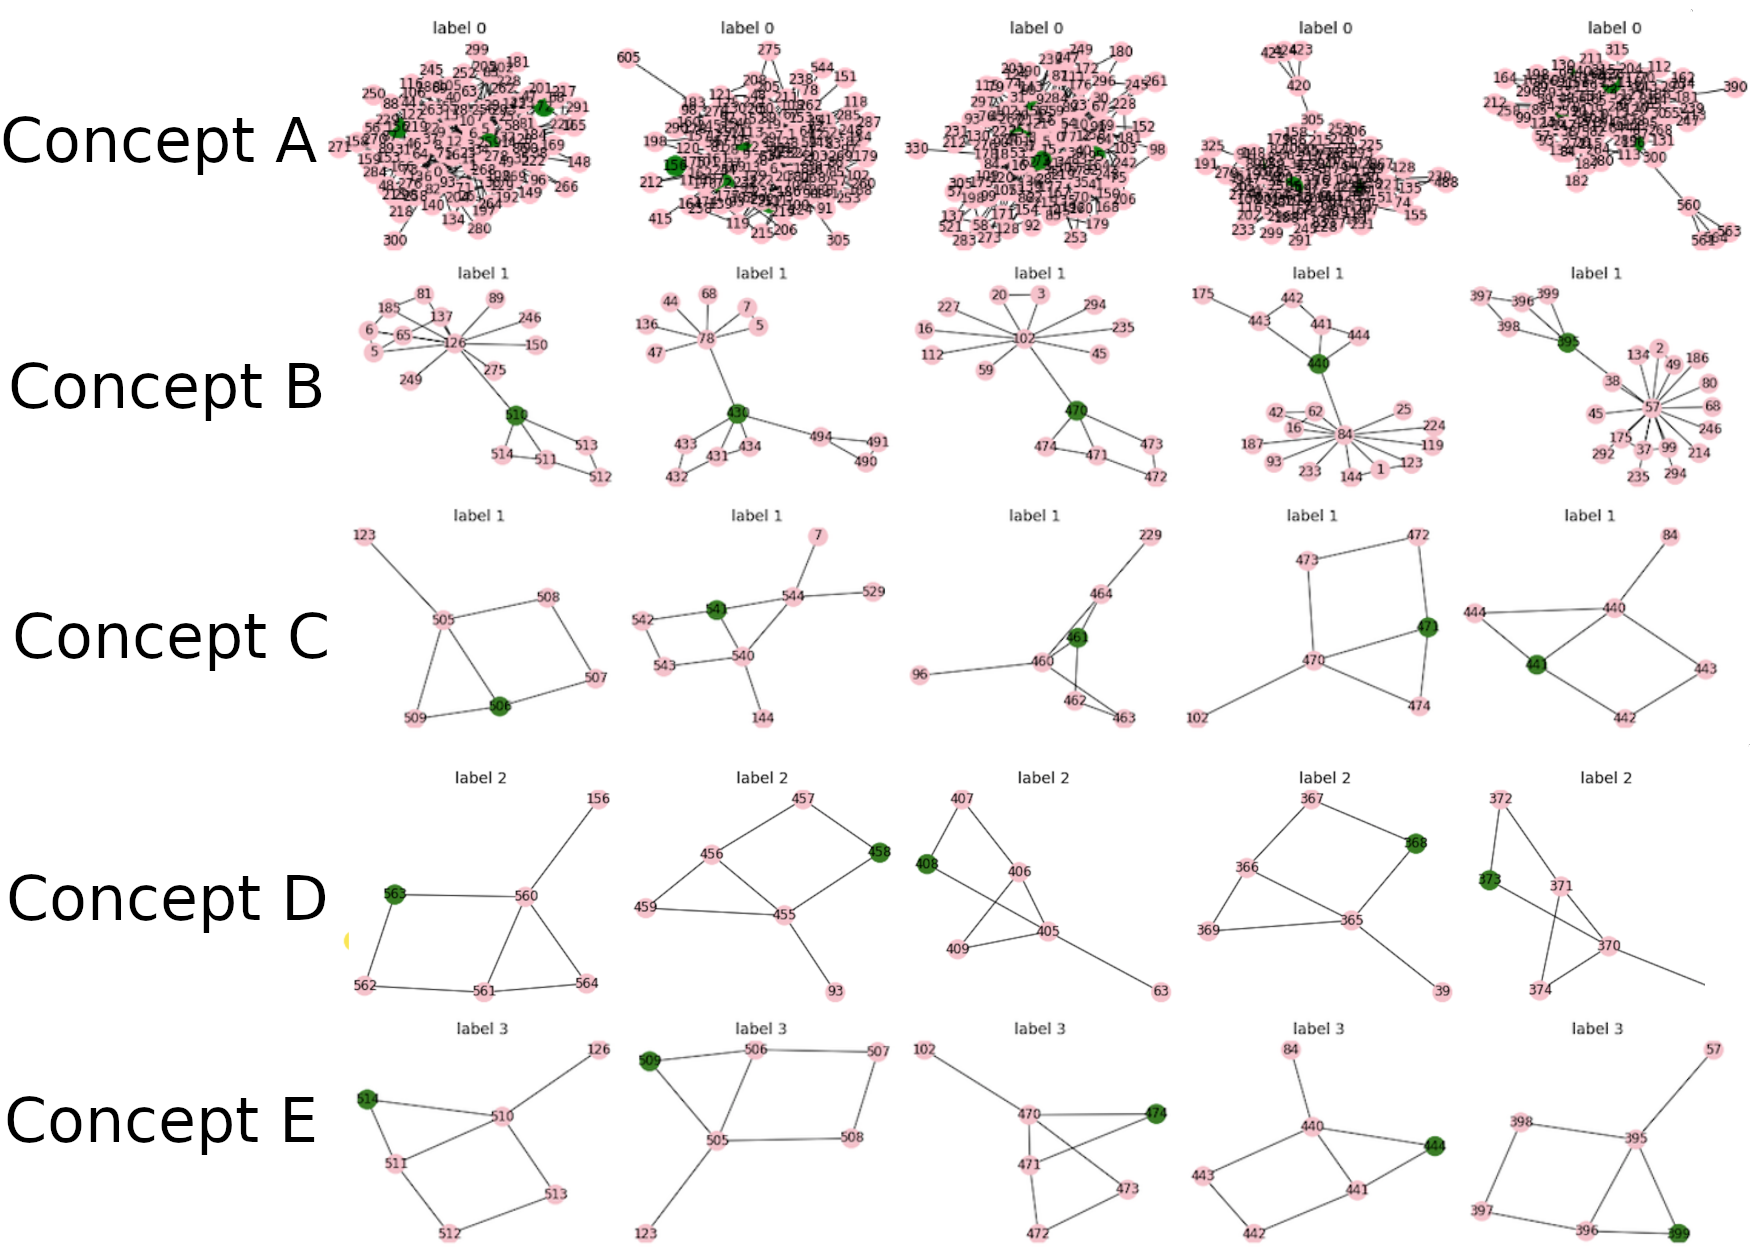
\includegraphics[width=0.45\textwidth]{figures/Magister-BA-Shapes}
    \caption{A subset of concepts discovered for BA-Shapes from the best perfomring GCN model compared to those published in figures 2, 3, and 5 in \textit{Magister et al.}\cite{magister2021gcexplainer}. Green nodes highlight the node of interest and pink nodes highlight the neighbourhood used for inference. Each row represents an individual concept.}
    \label{fig:GCN-BA-Shapes}
\end{figure}

%\fig{GCN-BA-Shapes}{A subset of concepts discovered for BA-Shapes from the best perfomring GCN model. Green nodes highlight the node of interest and pink nodes highlight the neighbourhood used for inference. Each row represents an individual concept.}
%
%\fig{Magister-BA-Shapes}{A subset of the BA Shapes concepts discovered in figures 2, 3 and 5 from \textit{Magister et al.}\cite{magister2021gcexplainer} to demonstrate the full range of labels. Each row represents an individual concept, the same colour system is used as fig. \ref{fig:GCN-BA-Shapes}.}

Figure \ref{fig:GCN-BA-Shapes} presents a comparison of BA Shapes concepts reproduced by the best performing GCN model and hose published in \textit{Magister et al.}
Concept 1 and A are included to demonstrate that the model does identify the base graph.
The remaining concepts demonstrate the 3 other labels associated with the house motif, as discussed in \Sref{sec:synth}.
All the published concepts have an equivalent concept in the reproduced concepts.
In both results the edge attaching the house motif to the base graph is important to the classification of the nodes.
The same distinction between concepts 2 and 3 as concepts B and C representing ``inside'' and the ``outside'' nodes respectively is also present in both.
%Notice that in both concept 2 and B the  ``inside'' node clearly attaches to the Barabasi-Albert base graph.
%This distinction is also present in concept 4 and D, with both the published and reproduced concepts focusing on the ``inside'' bottom node.

In both cases, and as expected given the concept purity scores, the concepts related to the motifs are almost completely pure with the exception of concept 1 and B.
Additionally, all the nodes in the house motif have a unique concept where applicable and this leads to the high completeness score.

Given the visual similarity in concepts between the published and reproduced results I consider the implementation of GCN to be accurate.
Examples of the other datasets are available in \Aref{app:concepts}.

\section{Comparison of Accuracy}
\label{sec:comp-acc}
\begin{table}
    \centering
    \begin{tabular}{c|c}
        \textbf{Dataset} & \textbf{Accuracy} \\
        \midrule
        BA Shapes       & 61.4\% $\pm$ 3.3 \\
        BA Grid         & 72.4\% $\pm$ 1.6 \\
        BA Community    & 20.6\% $\pm$ 1.5 \\
        Tree Cycles     & 50.5\% $\pm$ 4.2 \\
        Tree Grid       & 59.2\% $\pm$ 1.6 \\
    \end{tabular}
    \caption{Test accuracy in \% of SGC on each of the synthetic datasets using the hyperparameters in table \ref{tab:SGC-params}. As per \textit{Wu et al.}\cite{wu2019simplifying} outliers are removed as defined in \note{reference when complete}.}
    \label{tab:GCN-acc}
\end{table}



Table \ref{tab:SGC-acc} demonstrates the mean accuracies achieved by each of the SGC models using the hyperparameters in \ref{tab:SGC-params}.
As a comparison the accuracies achieved by GCN are presented beside them.
The performanace of SGC is very poor and so random guesses are included to demonstrate this.

\paragraph{Compared to GCN}
the accuracies achieved by SGC are significantly worse and go against \textit{Wu et al.}'s claim that SGC can match GCN perfomance.
In the majority of cases the accuracy achieved by SGC is roughly $50\%$ less than that achieved by GCN.
BA Grid, the highest performing dataset, achieves $72.4\%$ accuracy which is still $27.1\%$ less than GCN.
%does SGC achieve a good accuracy in comparison to GCN though even here the difference in accuracy is $27.1$\%.

These poor results suggest that the graph structure awareness of SGC is far worse than that of GCN as labels are based only on graph structure.
This is also an explanation for why SGC is able to surpass the accuracy of GCN in the Planetoid\cite{kipf2016semi} datasets as these datasets rely heavily on node representations.

\paragraph{Compared to random guesses}
SGC does not perform significantly better except in the cases of BA Shapes and BA Grid.
In the cases of the Tree datasets this can be attributed to the sparsity of the base graph where the motif structure and BST structure share similar connectivity.

In comparison the dense BA graph allows for a better distinction between the motifs and the base graph.
This distinction is attributed to the degree normalisation demonstrated in equation \ref{eq:GCN-as-GNN}.
This advantage is not present in BA Community the two communities and the possibility of a motif having multiple connections to different base graphs.

These results are not due to poor hyperparameter selection as demonstrated in \Aref{app:hyperparameters} and discussed in \Sref{sec:hyperparameters}.
Instead the explanation for the poor performance is due to the lack of proper graph structure awareness.

\paragraph{Comparison of parameters}
Given that SGC uses a single classifier layer compared to GCNs multiple layers there is a large discrepancy in the number of parameters\footnote{SGC has roughly 40 parameters compared to GCN with $>$1000 for BA Shapes.}.
However, increasing the parameters for SGC by either increasing the node feature size or adding a \emph{multi-layer perceptron}(MLP)\footnote{The use of an MLP classifier also introduces non-linearity though in this case the model does not improve. Non-linearity and parameters on there own are not sufficient.} with the same hidden layers as the GCN model results in no substantial change to accuracy.

No MLP model is added before the SGC pre-computation step as this defeats the point of linearisation.
This is the main drawback of SGC as it cannot manipulate the node representations except through filter application.
These claims are further explored in \Sref{sec:comp-concept}.

\section{Comparison of concepts}
\label{sec:comp-concept}

To achieve the \ref{crit1}$^{st}$ and \ref{crit3}$^{rd}$ success criterion concepts need to be extracted from SGC and compared to GCN concepts.
However, as stated before, concept extraction and analysis is only suggested for models that achieved $95$\% or higher on synthetic datasets by \textit{Ying et al.}\cite{ying2019gnnexplainer}.
As demonstrated in \Sref{sec:comp-acc} SGC does not reach this value only reaching $72.4$\% in the best case.

However, though the concepts will not be meaningful to explain how SGC reasons they will still provide insight into the claims in \Sref{sec:comp-acc}.
Furthermore, the concepts highlight the shortcomings of SGC when it comes to graph structure awareness.
For this reason the analysis of the concept scores is limited but the qualitative concept analysis provides insight into where SGC fails.

\paragraph{Success criterion}
Table \ref{tab:SGC-acc} demonstrates and implementation of SGC trained on the synthetic datasets with tables \ref{tab:SGC-completeness} and \ref{tab:SGC-purity} showing concept extraction.
Figures \ref{fig:SGC-BA-Shapes} and \ref{fig:BA-Community} visualise the extracted concepts from the relevant SGC model. These fulfill the \ref{crit1}$^{st}$ success criterion.

Table \ref{tab:SGC-completeness} and \ref{tab:SGC-purity} also include a comparison to the scores achieved by GCN.
\Sref{sec:comp-concept} includes a detailed analysis of the concepts extracted for SGC and comparison to those extracted for GCN.
These fullfil the \ref{crit3}$^{rd}$ success criterion.

\subsection{Quantitative analysis}
\label{sec:quant}
\paragraph{Completeness}
\begin{table}
    \centering
    \begin{tabular}{c|c|c}
        \textbf{Dataset} &
        \textbf{SGC} &
        \textbf{GCN} \\
        \midrule
        BA Shapes       & 0.882 & 0.964 \\
        BA Grid         & 0.843 & 1.000 \\
        BA Community    & 0.264 & 0.678 \\
        Tree Cycles     & 0.874 & 0.949 \\
        Tree Grid       & 0.890 & 0.965 \\
        \midrule
        Mutagenicity    & 0.537 & 0.967 \\
    \end{tabular}
    \caption{Concept completeness scores of SGC on each of the synthetic datasets using the hyperparameters in table \ref{tab:SGC-params} compared to the completeness scores of the equivalent GCN models.}
    \label{tab:SGC-completeness}
\end{table}



Table \ref{tab:SGC-completeness} demonstrates the completeness scores achieved by SGC compared to GCN and as expected, by the low accuracy achieved by SGC in table \ref{tab:SGC-acc}, they are consistently lower than the equivalent GCN models.
However, the resulting completeness scores are close to the GCN scores except in the case of BA Community.

The high completenes scores are due to the fact that completeness relates to importance of concepts and not the performance of the model.
The relatively high completeness scores for SGC signify that the concepts that SGC produces have some relevance to the class of a node.
However, as demonstrated by table \ref{tab:SGC-completeness}, this relevance is not as strong as that in GCN.

\paragraph{Purity}
\begin{table}
    \centering
    \begin{tabular}{c|ccc|c}
        \multirow{2}{*}{\textbf{Dataset}} &
        \multicolumn{3}{c}{\textbf{SGC}} & \\
        & \textbf{Max.} & \textbf{Min.} & \textbf{Mean} & \multirow{-2}{*}{\textbf{GCN}}\\
        \midrule
        BA Shapes       & 0.0 & 4.0 & 0.8 (5) & 0.000 (4) \\
        BA Grid         & 0.0 & 0.0 & 0.0 (2) & 0.000 (2) \\
        BA Community    & 0.0 & 6.0 & 4.0 (4) & 5.600 (3) \\
        Tree Cycles     & 0.0 & 6.0 & 1.0 (6) & 4.391 (9) \\
        Tree Grid       & 0.0 & 7.0 & 3.3 (10) & 1.417 (6) \\
    \end{tabular}
    \caption{Concept purity of SGC on each of the synthetic datasets using the hyperparameters in table \ref{tab:SGC-params} compared to the average purity achieved by the equivalent GCN model. The brackets represent the number of concepts considered for purity, as per \Sref{sec:evaluation} these are graphs with less than 13.}
    \label{tab:SGC-purity}
\end{table}



Table \ref{tab:SGC-purity} includes the purity scores achieved by the best performing SGC models compared to the corresponding GCN models.
As discussed in \Sref{sec:GCN-reproduction} the values for purity are likely to be very erratic and not well suited for direct comparison.
Given this erratic behaviour the values for purity between the two approaches are somewhat correlated with SGC achieving fairly pure concepts.

However, the inclusion of the number of concepts considered when calculating purity demonstrates the limitation of this method of comparison.
Due to the base graphs a number of concepts contain more than 13 nodes and therefore are not considered.
Thus the pure concepts of BA Grid are not representative of all the concepts extracted.

Overall, this demonstrates that though SGC does not perform as well as GCN it produces concepts that are as coherent as GCN.

\subsection{Qualitative analysis}
\label{sec:concept-analysis}

\paragraph{BA Shapes}
\fig{SGC-BA-Shapes}{A subset of concepts extracted from the best performing SGC model. The subset includes both pure and impure concepts. The same colour scheme as fig. \ref{fig:GCN-BA-Shapes} is used.}

Figure \ref{fig:SGC-BA-Shapes} visualises a subset of the concepts extracted for SGC on BA Shapes.
Concepts 1 to 4 demonstrate the purer concepts extracted for SGC with concepts 5 to 7 representing the more common impure concepts.
Concept 5 demonstrates a shortcoming of calculating purity as this is considered a ``pure'' concept as the Barabasi-Albert graphs, having more than 13 nodes, are not considered. 
As with GCN, concept 1 demonstrates that SGC is able to identify the base graph.

Concepts 2, 3 and 4 demonstrate that SGC can identify pure concepts with important graph structure components.
These concepts can be directly compared to concepts 3, 2 and 4 in figure \ref{fig:GCN-BA-Shapes} respectively.
As with GCN the attaching arm is important to the classification of the nodes and there is some distinction between ``inside'' and ``outside'' nodes.
However, as can be seen in concept 2, this distinction is not as strong as GCN.

Concepts 5, 6 and 7 demonstrate the impure concepts that are extracted from SGC.
This is the major shortcoming of SGC it cannot consistently distinguish between the base graph and the motif.
%Given that the nodes of interest in house motif are all consistent across these concepts suggests that there is an element of structure being identified.
The problem is that SGC is unable to discern between structures that produce similar node representations.

These observations are hypothesised to be a result of limited learnable influence on node representations in SGC.
Though equation \ref{eq:theta} suggests that the GCN node manipulation should be preserved the reality is that only the final filter output is manipulated.
This observation leads to the extension presented in \Sref{sec:Jump-SGC} allowing SGC to access individual filter applications.

\paragraph{BA Community}
\begin{figure}
    \centering
    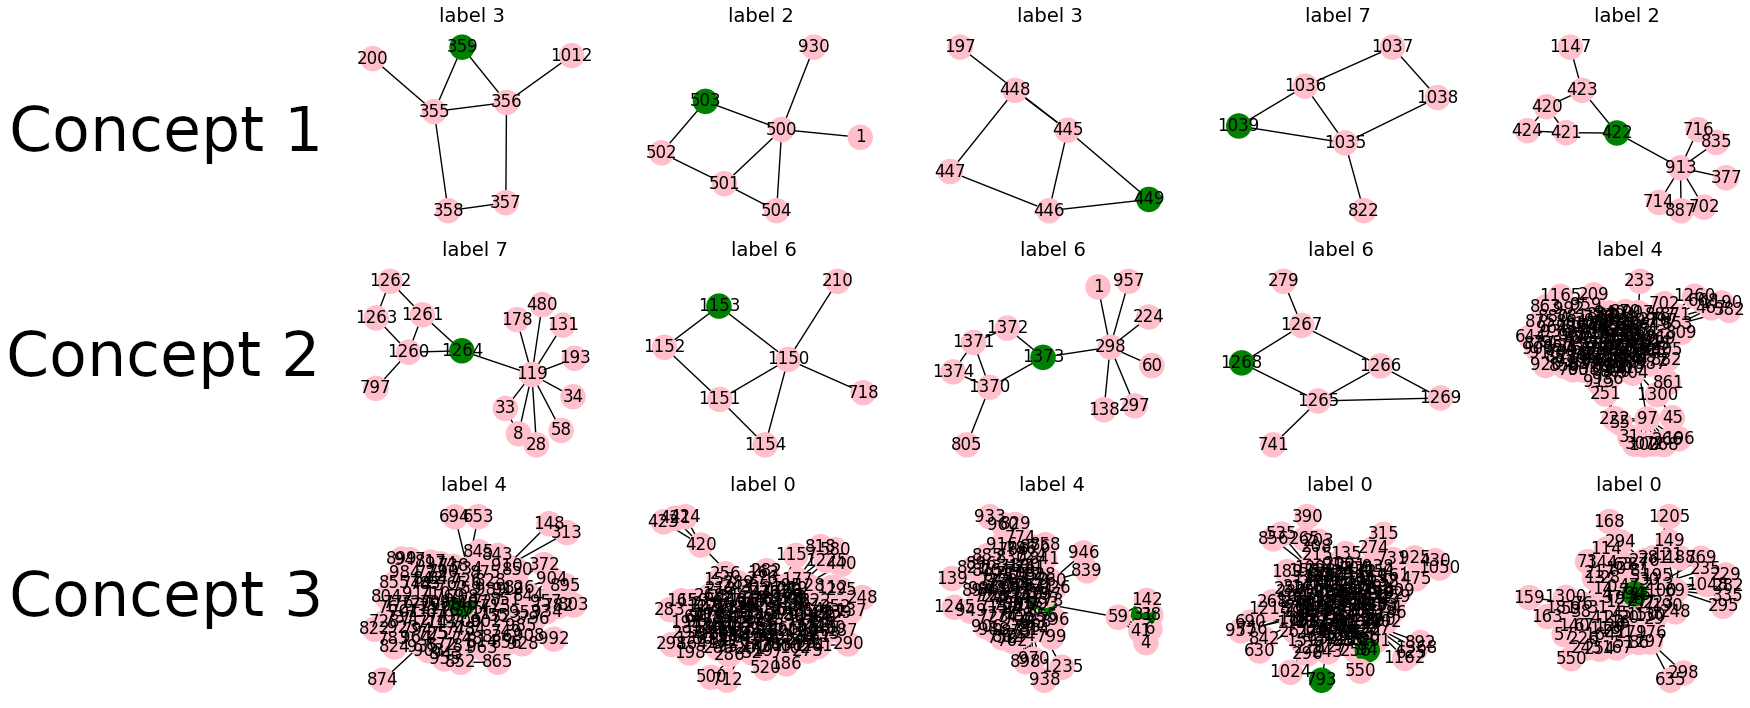
\includegraphics[width=0.75\textwidth]{figures/SGC-BA-Community}
    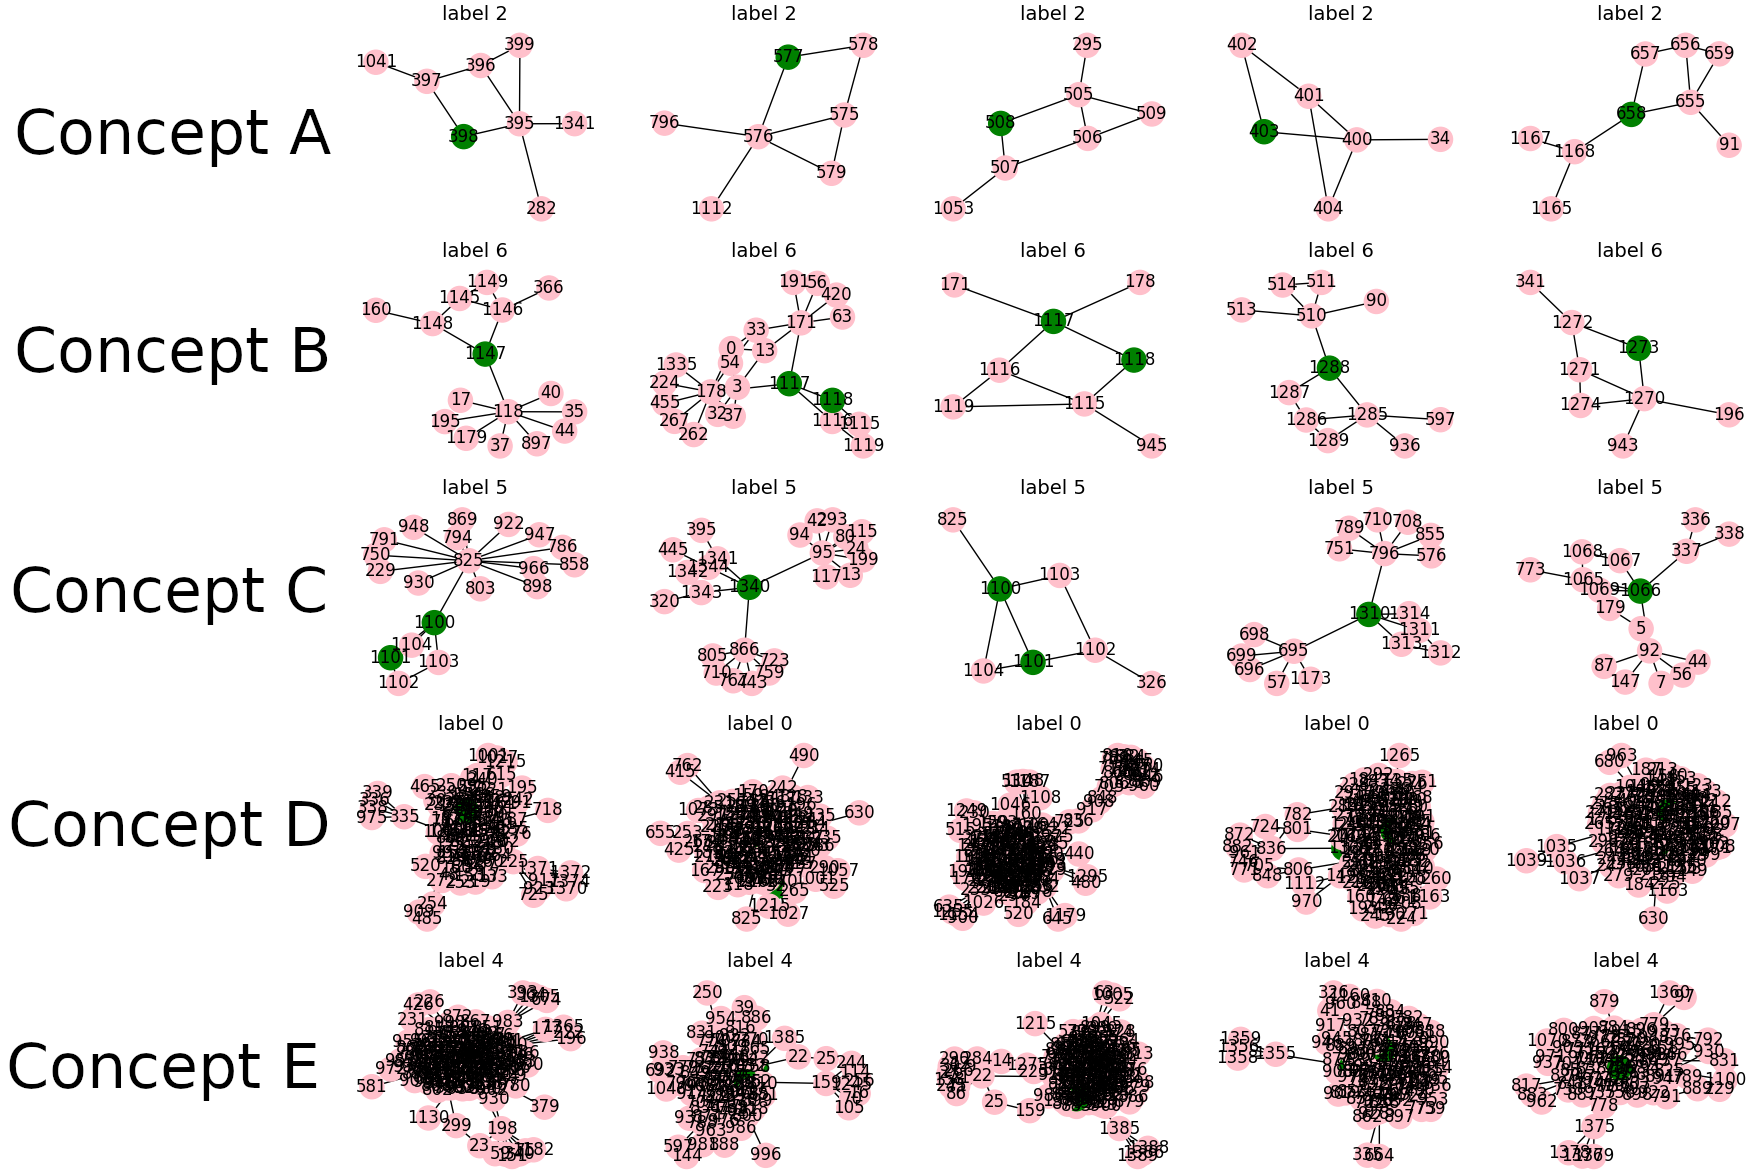
\includegraphics[width=0.75\textwidth]{figures/GCN-BA-Community}
    \caption{Comparison of SGC and GCN concepts for BA Community demonstrating the poor graph structural inference of SGC. The numbered concepts are a subset of SGC concepts and the lettered concepts are GCN concepts. The colour scheme is the same as fig. \ref{fig:GCN-BA-Shapes}.}
    \label{fig:BA-Community}
\end{figure}

Figure \ref{fig:BA-Community} highlights the inability of SGC to accurately discern graph structure where GCN demonstrate accurate graph structure awareness.
Concepts 1, 2 and 3 demonstrate the purer concepts for SGC trained on BA Community and Concepts A to E represent the equivalent concepts for GCN.

As discussed SGC may be able to identify graph structure, as shown in concepts 1 and 2, however concept 1 highlights the fact that SGC cannot determine which part of the graph structure a node is.
Comparatively concepts A, B and C show similar structures except consistent labels across the concept.

Furthermore, concept 2 groups nodes from the second community\footnote{labels 4, 5, 6 and 7.} together not nodes with the same graph structure.
In comparison, GCN is able to discern between members in the same community demonstrated by concepts B and C
Additionally, GCN can distinguish between different communities as concepts A and B represent the same node in the house motif but different communities.
%This erroneous behaviour is not standard as concept 3 highlights how the Barabasi-Albert subgraphs from separate communities are grouped together.
GCN treats the two communities different regardless of structural similarity which is clear in concepts D and E compared to concept 3.

Overall SGC is able to infer basic graph structure or group nodes into communities but is unable to achieve fine-grained awareness.
Though particularly apparent in BA Community these behaviours of SGC effect the performance on other datasets.

\subsection{Summary}
%The low accuracy of SGC means that the data present in tables \ref{tab:SGC-completeness} and \ref{tab:SGC-purity} does not carry much meaning.
%However, table \ref{tab:SGC-completeness} does suggest that SGC does not produce useful concepts even though table \ref{tab:SGC-purity} suggests that these concepts are coherent.

SGC is not as capabale as GCN when dealing with synthetic datasets where graph structure is important.
Table \ref{tab:SGC-acc} demonstrates poor performance across the full range of synthetic datasets and tables \ref{tab:SGC-completeness} and \ref{tab:SGC-purity} show the corresponding low concept scores.
Attempts to improve the performance by increasing the parameters of SGC have resulted in no substantial improvement to accuracy or concept score.

The concepts extracted from SGC across the datasets demonstrate a lack of graph structure awareness which is a key feature of any GNN.
Figures \ref{fig:SGC-BA-Shapes} and \ref{fig:BA-Community} highlight the impure and unstructured concepts typical of SGC.
These results suggest that the linearisation of GCN clearly does not maintain the graph capabilities of GCN contrary to the results and claims of \textit{Wu et al.}.

However, as discussed in \Sref{sec:comp-acc}, the lack of influence that SGC has on node representations is likely the cause for low performance.
SGC can only manipulated the final convolution node representations which provide limited insight into the structure of the graph.
Extensions described in \Sref{sec:extension-imp} and evaluated in \Sref{sec:extension-eval} aim to combat this to provide a fairer comparison between the two models.

\section{Extensions}
\label{sec:extension-eval}
\subsection{Evaluation}
All the extensions explored focus on improving the ability of SGC or expanding the functionality of the model.
Therefore to evaluate the success of these attempts the models are evaluated using the same techniques used in \ref{sec:evaluation}.
As these are extensions a smaller subset of the graph datasets are considered looking mainly at BA Shapes, as the best performing dataset, and BA Community, as the worst.

\subsection{SGC graph classification}
\label{SGC-graph}
\fig{SGC-Mutagenicity}{Concepts from SGC and GCN for Mutagenicity comparing the complexity of the inferred graph structure. The numbered concepts are a subset of SGC concepts and the lettered concepts are a subset of GCN. The colour scheme matches standard chemical colours.}

Tables \ref{tab:SGC-acc}, \ref{tab:SGC-completeness} and \ref{tab:SGC-purity} already include the results achieved by SGC on Mutagenicity.
The same quantitative analysis presented in \Sref{sec:quant} can be applied to the results achieved by SGC.
This suggests that the source of the graph data is not the issue, even though SGC performed well on Planetoid\cite{Fey/Lenssen/2019}.
As discussed in \Sref{sec:comp-acc} the cause for the discrepancy is due to Planetoid\cite{Fey/Lenssen/2019} being focused on node representation.
%Comparatively, Mutagenicity is both node representation and graph structure focused due to the nature of molecules.

Figure \ref{fig:SGC-Mutagenicity} further highlights the shortcomings of SGC compared to GCN.
Concepts 1, 2 and 3 focus on the inclusion of a single atom or small molecule structure wheres A, B and C demonstrate complex multi-atom structures.
Concepts 1 and 2 suggest identification structure though consistently focus on single atoms whereas concepts A and B show consistent multi-atom structures.
In the extreme concept 3 highlights the focus on grouping by atom, the major consistent feature the chlorine atom.
In comparison, concept C highlights how GCN is able to identify very large structures, two cyclic rings are consistently identified across all examples.

\subsection{SGC and GCN mixed model}
\label{sec:SGCN}

\begin{figure}
    \centering
    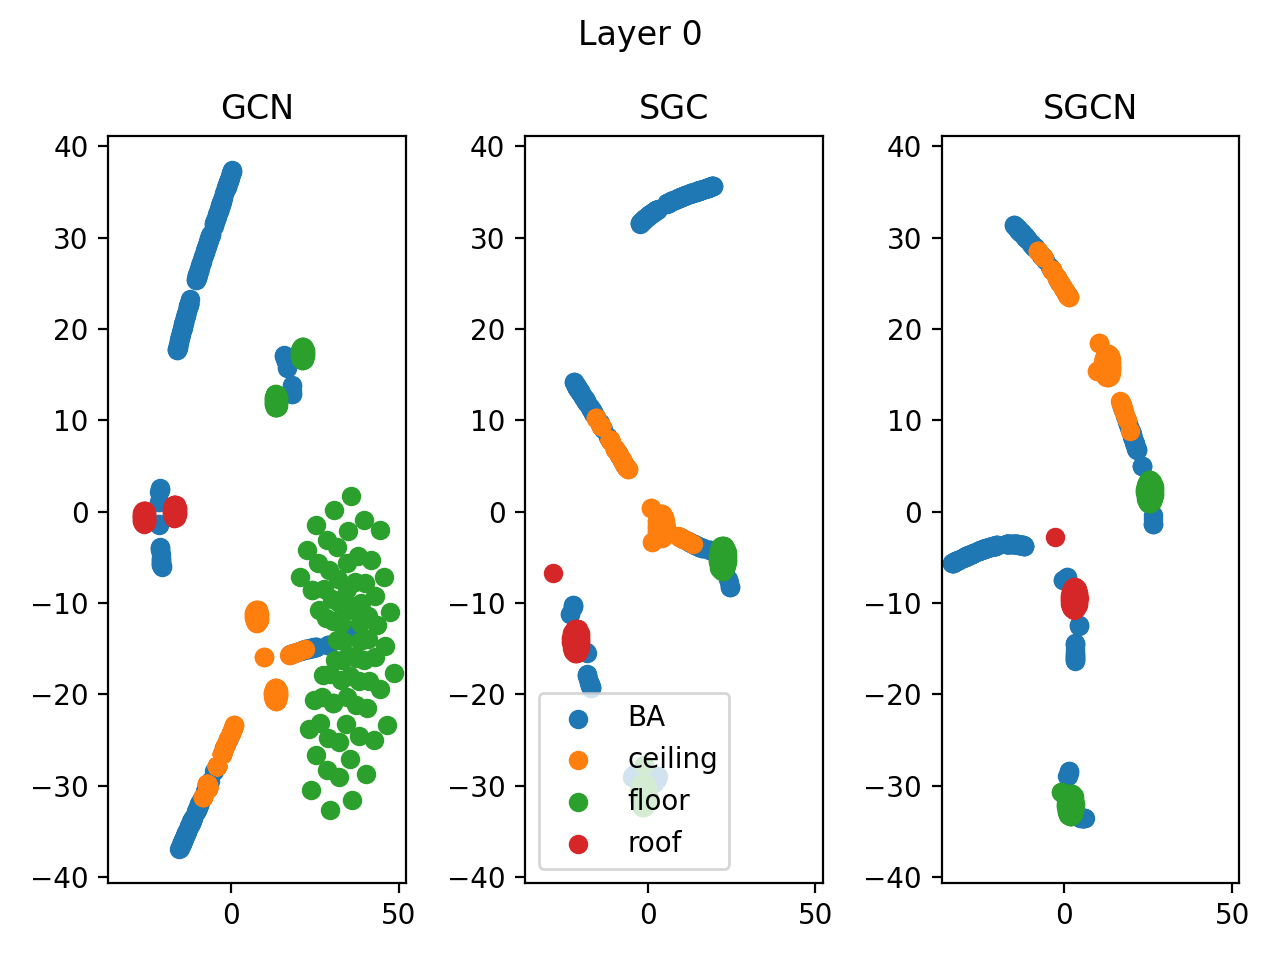
\includegraphics[width=0.40\textheight]{figures/SGCN-latent-space-0}
    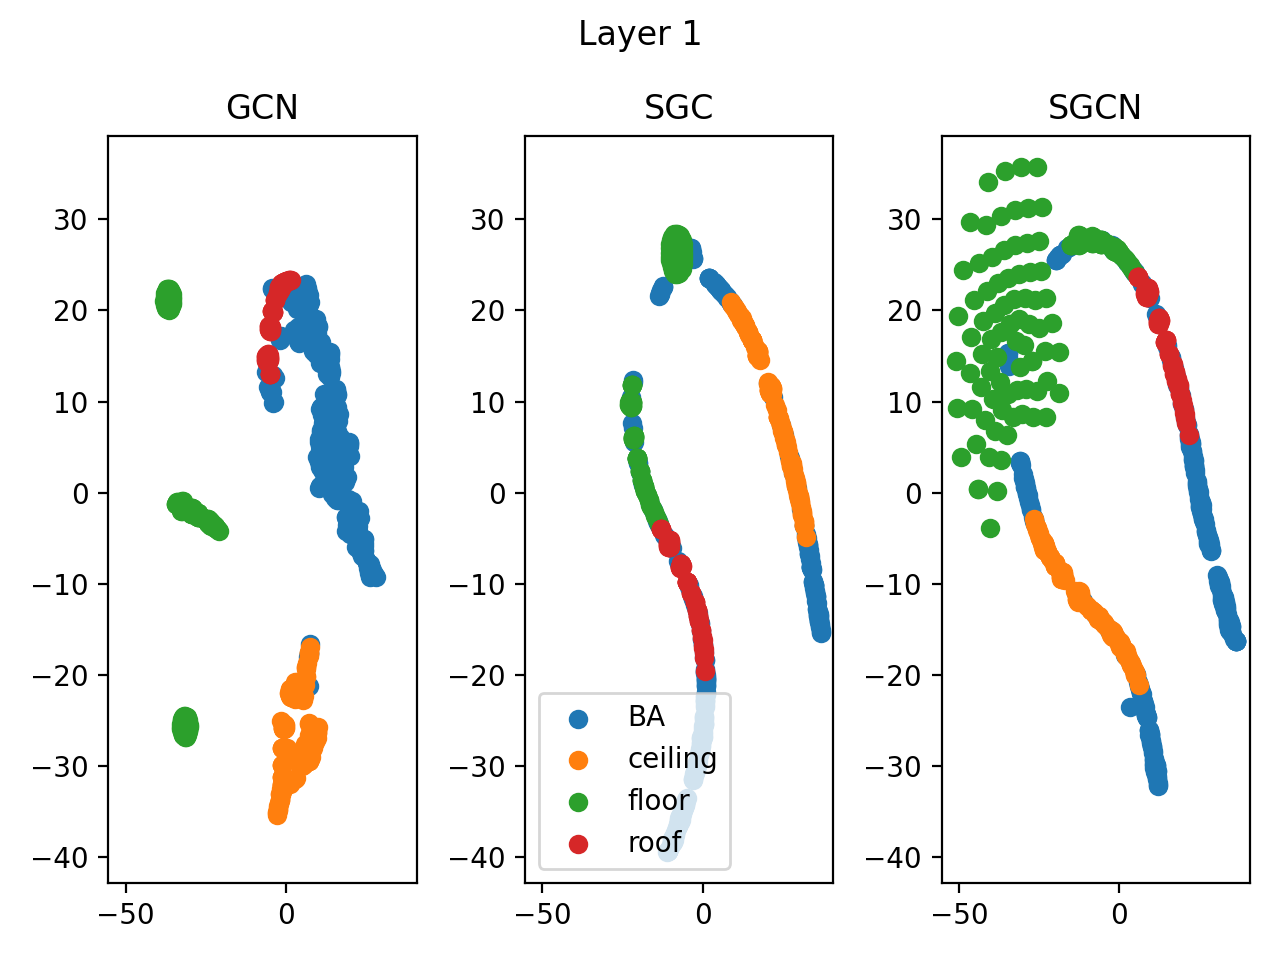
\includegraphics[width=0.40\textheight]{figures/SGCN-latent-space-1}
    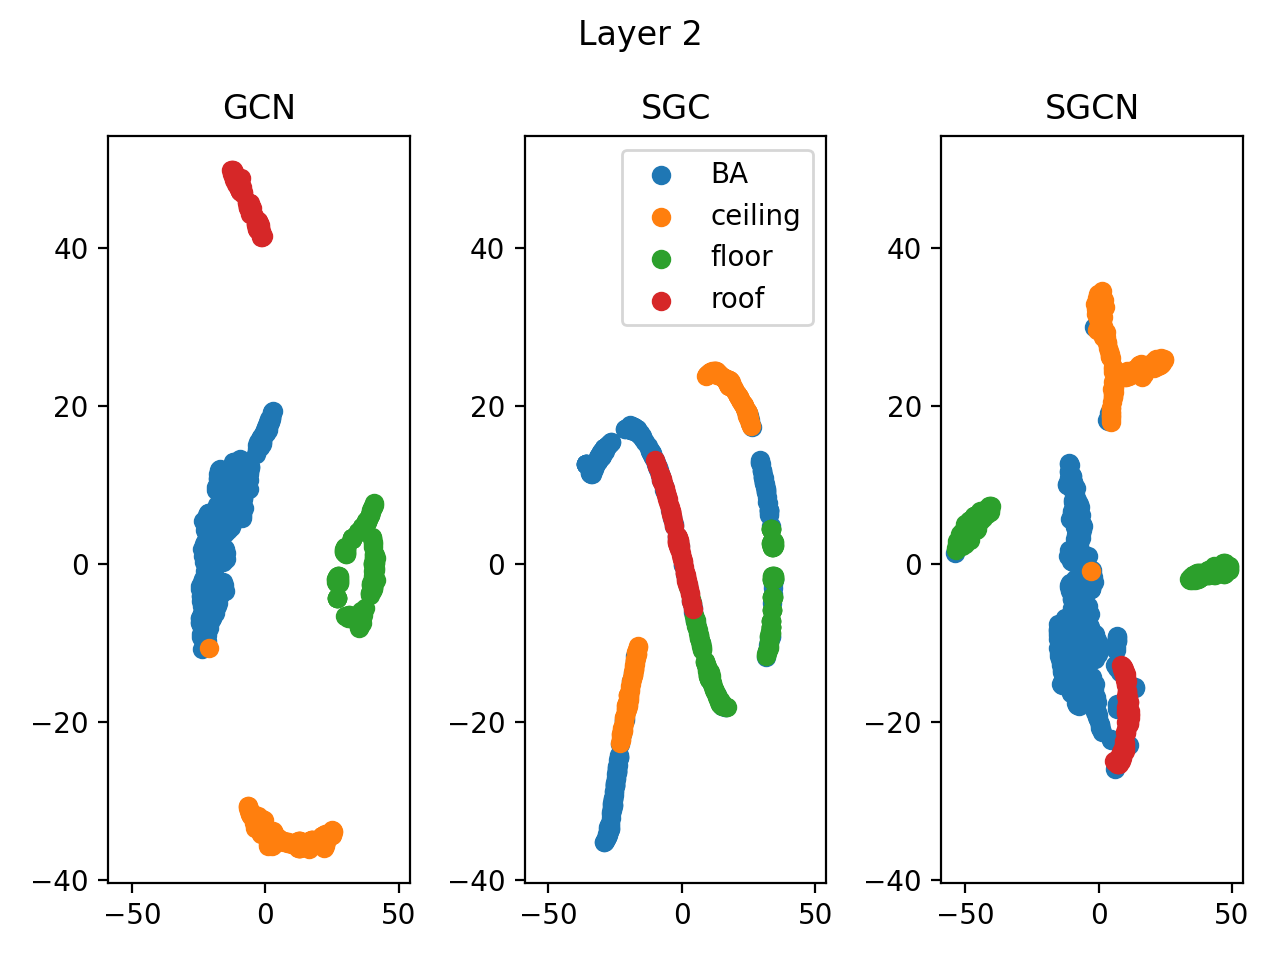
\includegraphics[width=0.40\textheight]{figures/SGCN-latent-space-2}
    \caption{The 2D t-SNE reduced latent space of the three different models for each GNN layer (that is ignoring the classifier). Concepts are calculated with the same number of clusters and receptive field. The labels are based on true labels not inferred labels for a better comparison between the models.}
    \label{fig:SGCN-latent-spaces}
\end{figure}

%\fig{SGC-GCN-latent-space}{The 2D t-SNE reduced latent space of the first layer where SGC and GCN activations are most similar based on adjusted mutual information of their concepts. Concepts are calculated with the same number of clusters and receptive field.}
%\fig{SGCN-SGC-latent-space}{The 2D t-SNE reduced latent space of the second layer where SGCN and SGC activations are most similar based on adjusted mutual information of their concepts. Concepts are calculated with the same number of clusters and receptive field.}
%\fig{SGCN-GCN-latent-space}{The 2D t-SNE reduced latent space of the final (third) layer where SGCN and GCN activations are most similar based on adjusted mutual information of their concepts. Concepts are calculated with the same number of clusters and receptive field.}
\begin{table}[h]
    \centering
    \captionsetup{width=.9\textwidth}
    \begin{tabular}{c|c|cc}
        \textbf{Dataset} & \textbf{SGCN} & \textbf{SGC} & \textbf{GCN} \\
        \midrule
        BA Shapes       & 95.6\% $\pm$ 3.0 & 61.4\% $\pm$ 3.3 & 98.0\% $\pm$ 2.2 \\
    \end{tabular}
    \caption{Test accuracy in \% of SGCN on BA Shapes where the first layer is SGC precomputaion and the remaining two layers are GCN layers. The results achieved by SGC and GCN run for the same number of epochs are added as comparison.}
    \label{tab:SGCN-acc}
\end{table}


\begin{table}
    \centering
    \begin{tabular}{c|c|cc}
        \textbf{Model} & \textbf{Layer 1} & \textbf{Layer 2} & \textbf{Layer 3} \\
        \midrule
        GCN     & 0.736 & 0.743 & 0.926 \\
        SGC     & \underline{0.800} & 0.757 & 0.700 \\
        \midrule
        SGCN    & \underline{0.800} & \textbf{0.764} & \textbf{0.971} \\
    \end{tabular}
    \caption{Completeness scores for each of the layers of SGCN trained on BA Shapes where the first layer is SGC precomputaion and the remaining two layers are GCN layers. The results achieved by SGC and GCN run for the same number of epochs are added as comparison.}
    \label{tab:SGCN-completeness}
\end{table}



As the process of finding the optimal model, training and evaluating requires many steps only BA Shapes is considered.
Figure \ref{fig:SGCN-latent-spaces} shows the t-SNE reduced latent space of each layer and model.
Tables \ref{tab:SGCN-acc} and \ref{tab:SGCN-completeness} demonstrate the results achieved by SGCN in both accuracy and concept completeness.

Layer 0 in fig. \ref{fig:SGCN-latent-spaces} demonstrates the first layer which has the highest AMI between GCN and SGC.
The similarity is not very high but is significantly higher than the similarity between SGC and GCN for the remaining layers.
This does present a potential issue in combining models where no significant mutual information is present.

Layer 1 in fig. \ref{fig:SGCN-latent-spaces} demonstrates that the second layer of SGCN is very similar to that of SGC.
This is due to the previous layer being an SGC layer and so the GCN layer applied to a different feature space.
The spread green labelled nodes (representing the ``floor'') is present in the GCN layer 0 and SGCN layer 1 demonstrating a mixture of representation.

Layer 2 in fig. \ref{fig:SGCN-latent-spaces} shows that the final layer of SGCN has a latent space that is very similar to that of GCN.
Given the increase in performance by SGCN this latent space likely to be better.

Though SGCN does not surpass the performance of GCN as shown in table \ref{tab:SGCN-acc} it is able to surpass it in completeness score highlighted in table \ref{tab:SGCN-completeness}.
This happens across all layers (noting that the first layer is identical to the SGC layer) and highlights a major benefit of the model.
GCN takes all 3 layers to reach a high completeness score whereas SGC starts high but then decreases as more layers are added.
By combining the layers the completeness score to remains high throughout.

An analysis of the concepts extracted for SGCN are presented in \Sref{app:concepts}.

\subsection{Jumping knowledge SGC}
\label{sec:Jump-SGC}

\begin{table}
    \centering
    \begin{tabular}{c|c|cc}
        \textbf{Dataset} & \textbf{JSGC} & \textbf{SGC} & \textbf{GCN} \\
        \midrule
        BA Shapes       & 78.2\% $\pm$ 3.2 & 61.4\% $\pm$ 3.3 & 98.0\% $\pm$ 2.2 \\
        BA Community    & $\pm$ & 20.6\% $\pm$ 1.5 & 86.3\% $\pm$ 3.3 \\
    \end{tabular}
    \caption{Test accuracy in \% of JSGC on a subset of synthetic datasets using the hyperparameters in table \note{reference when complete}. Each experiment is run until convergence. Results from SGC and GCN are provided as a comparison.}
    \label{tab:SJGC-acc}
\end{table}


\begin{table}[h]
    \centering
    \captionsetup{width=.9\textwidth}
    \begin{tabular}{c|c|cc}
        \textbf{Dataset} &
        \textbf{JSGC} &
        \textbf{SGC} &
        \textbf{GCN} \\
        \midrule
        BA Shapes       & 0.943 & 0.882 & 0.964 \\
        BA Community    & \textbf{0.704} & 0.264 & 0.678 \\
    \end{tabular}
    \caption{Concept completeness scores of JSGC on a subset of the synthetic datasets using the hyperparameters in table \ref{tab:JSGC-params} compared to the completeness scores of the equivalent SGC and GCN models. Each model is run until convergence and the best performing model selected for concept extraction.}
    \label{tab:JSGC-completeness}
\end{table}


\begin{table}[h]
    \centering
    \captionsetup{width=.9\textwidth}
    \begin{tabular}{c|ccc|cc}
        \multirow{2}{*}{\textbf{Dataset}} &
        \multicolumn{3}{c|}{\textbf{JSGC}} & \\
        & \textbf{Max.} & \textbf{Min.} & \textbf{Mean} & 
        \multirow{-2}{*}{\textbf{SGC}} &
        \multirow{-2}{*}{\textbf{GCN}}\\
        \midrule
        BA Shapes       & 0.0 & 0.0 & 0.0 (2) & 0.8 (5) & 0.000 (4) \\
        BA Community    & 4.0 & 16.0 & 9.4 (7) & 4.0 (4) & 5.600 (3) \\
    \end{tabular}
    \caption{Concept purity of JSGC on a subset of the synthetic datasets using the hyperparameters in table \ref{tab:JSGC-params} compared to the average purity achieved by the equivalent SGC and GCN model. The brackets represent the number of concepts considered for purity, as per \Sref{sec:evaluation} these are graphs with less than 13.}
    \label{tab:JSGC-purity}
\end{table}


\fig{JSGC-latent-space}{The final layer in the GCN, SGC and JSGC architectures for BA Shapes. As shown JSGC has clear clusterings for the different labels similar to GCN but the clustering is not as pronounced likely leading to the lower accuracy. In comparison SGC exhibits no clear clustering.}

Tables \ref{tab:JSGC-acc}, \ref{tab:JSGC-completeness} and \ref{tab:JSGC-purity} show the results achieved by JSGC.
Overall these demonstrate that JSGC does outperform SGC significantly and is more comparable to GCN.
The accuracy achieved by JSGC is still lower than the the 95\% suggested by \textit{Ying et al.}\cite{ying2019gnnexplainer} but significantly better.
This improvement is seen in table \ref{tab:JSGC-completeness} as the completeness scores are closer to 1 with BA Community producing better performing concepts than GCN.\footnote{This is partially a result of the concept parameters used. The high score signifies that good concepts are being utilised by the model but in this case the model still does not appear to be quite capable enough.}
The purity presented in table \ref{tab:JSGC-purity} is higher though more concepts were considered and BA Community is a very complex graph.

\fig{JSGC-BA-Community}{A subset of concepts from JSGC for BA Community demonstrating the improved graph structure awareness. The concepts are chosen to represent the GCN concepts presented in \ref{fig:BA-Community}. The colour scheme is the same as fig \ref{fig:GCN-BA-Shapes}.}

Figure \ref{fig:JSGC-BA-Community} highlights the improvements that JSGC has made compared to SGC.
Comparing these concepts to those achieved by GCN presented in figure \ref{fig:BA-Community} shows a clear improvement.
Concepts 1 to 5 in fig. \ref{fig:JSGC-BA-Community} can be directly mapped to A to E in fig. \ref{fig:JSGC-BA-Community}.\footnote{A similar direct mapping was also achieved for BA Shapes.}
JSGC is now able to distinguish between the two communities highlighted by concepts 1 \& 2 and 3 \& 4.
Furthermore, within a community JSGC correctly distinguishes between the different nodes as concept 2, 3 and 4 show.
Most importantly all concepts, except for concept 1, show consistent labelling throughout, particularly in concept 3 where all nodes are ``outside'' nodes.

To further highlight the similarity between JSGC and GCN as well as the improvement on SGC figure \ref{fig:JSGC-latent-space} demonstrates the latent space of the concatenation layer in JSGC.
This demonstrates that JSGC has comparable graph structure awareness to GCN and does not require the non-linearity of GCN to achieve this.
The lower accuracy of JSGC still suggests that there are elements of GCN that are important to its success and generally GRL.
However, further studies into the importance of non-linearity in GRL are required.
